%Chapter 2

\renewcommand{\thechapter}{3}

\chapter{Comparing Metagenomic Assemblies}

\section{Abstract}
%\boldmath
The ever-decreasing costs of sequencing technology has led to a sharp increase in metagenomics projects over the past decade, allowing us to better understand the diversity and function of microbial communities found in the world around us.
The first step in these analyses is to perform
genome assembly to piece together the DNA fragments into complete, or
near complete, genomes.
%The first step in these analyses involves the use of tools called assemblers that piece together the DNA fragments into complete or near complete genome sequences.
Metagenomic assemblers inherit all the difficulties of traditional single genome assembly, but with the additional complexity of trying to resolve assemblies of closely related species with drastically varying abundances.
Assessing and comparing the quality of single genome assembly still relies on the availability of independently determined standards, such as manually curated genomic sequences.
These standards are often not possible in metagenomic projects, where a large portion of the organisms and strains are novel.
Thus, we must rely on \emph{de novo} methods for assessing and comparing assembly qualities.
Here we describe an extension to our \emph{de novo} LAP framework to evaluate metagenomic assemblies.
We will show that by modifying our likelihood calculation to take into account abundances of assembled sequences, we can accurately and efficiently compare metagenomic assemblies.
%We evaluate our extended framework on results generated from the Human Microbiome Project (HMP) and
We find that our extended LAP framework is able to reproduce results on data from the Human Microbiome Project (HMP) that closely match the reference-based evaluation metrics and outperforms other \emph{de novo} metrics traditionally used to measure assembly quality.
Finally, we have integrated our LAP framework into the metagenomic analysis pipeline MetAMOS, allowing any user to reproduce quality assembly evaluations with relative ease.
%Even without knowledge of the true reference sequences, our \emph{de novo} metric
%Here we introduce an extension to our LAP  \emph{de novo} probabilistic measure of assembly quality, which allows for an objective comparison of multiple assemblies generated from the same set of reads.
%We define the quality of a sequence produced by an assembler, as the conditional probability of observing the sequenced reads from the assembled sequence.


\section{Introduction}
The genome sequence of an organism is a vital resource for biologists trying to better understand its function and evolution.
Generating this sequence is not an easy task as modern sequencing technologies can only ``read'' small pieces of the genome.
These sequences, known as \emph{reads}, have to be pieced together by tools called assemblers using a collection of different heuristics since in almost all practical cases, assemblers cannot fully and accurately reconstruct the genome~\cite{myers1995,medvedev2007computability}.

Practical implementations of assembly algorithms (such as ABySS~\cite{ABySS}, SOAPdenovo~\cite{SOAPdenovo}, Velvet~\cite{Velvet}, etc.) return just an approximate solution that is often fragmented and contains numerous errors.
Ideally, further experiments would be performed manually to correct the hundreds to thousands of errors~\cite{salzberg2005misassemblies}, and fill in the gaps between the chunks of assembled sequences (called contigs)~\cite{nagarajan2010finishing}.
However, the additional cost and effort necessary to finish a genome is only justifiable for a few high-priority organisms (typically model organisms).
Recent technology advances have demonstrated automatically assembled finish-grade quality bacterial genomes~\cite{chin2013nonhybrid, koren2013reducing, ribeiro2012finished}. However, the majority of genomes sequences available today are considered to be in a ``draft'' state, with no clear indication of their respective quality, possibly impacting the conclusions and experiments done on their sequences.

Despite the unresolved challenges of clonal genome assembly, the decreasing costs of sequencing technology has led to a sharp increase in metagenomics projects over the past decade.
% have been sharply on the rise over the past decade,
These projects allow us to better understand the diversity and function of microbial communities found in the environment, including the ocean\cite{rusch2007sorcerer,wu2011stalking,yooseph2007sorcerer}, Arctic regions \cite{varin2012metagenomic}, other living organisms\cite{he2013comparative} and the human body\cite{gill2006metagenomic,peterson2009nih}.
Traditional \emph{de novo} genome assemblers have trouble assembling these datasets due to the presence of closely related species and and the need to distinguish between true polymorphisms and errors arising from the sequencing technology.
Metagenomic assemblers often use heuristics based on sequencing (Meta-IDBA \cite{peng2011meta} and MetaVelvet\cite{namiki2012metavelvet}) and k-mer (Ray Meta \cite{boisvert2012ray}) coverage to split the assembly graph into subcomponents that represent different organisms, then apply traditional assembly algorithms on the individual organisms.

As the number of metagenomic assemblers available to researchers continues to increase, the development of approaches for validating and comparing the output of these tools is of critical importance.
Despite the incremental improvements in performance, none of the assembler tools available today outperforms the rest in all cases (as highlighted by recent assembly
bake-offs GAGE\cite{salzberg2011gage} and Assemblathons 1~\cite{earl2011assemblathon} and 2~\cite{bradnam2013assemblathon}).
Different assemblers ``win'' depending on the specific downstream analyses, structure of the genome, and sequencing technology used.
These competitions highlight the inherent difficulty of assessing assembly quality -- where do you set the line between increased contiguity and decreasing accuracy of the resulting sequence?
Evaluating the trade-off between increased contiguity and errors is difficult even when there is a gold standard reference genome to compare to, which is not available in most practical assembly cases.
Thus, we are forced to heavily rely on \emph{de novo} approaches based on sequence data alone.
% (including global ``sanity checks,'' such as gene density, which is expected to be high in bacterial genomes).

One objective \emph{de novo} metric, that has been used to evaluate and compare assembly quality, is based on the likelihood that the observed reads are generated from the given assembly, which can be accurately estimated by modeling the sequencing process.
This metric was proposed by Gene Myers in his pioneering work in the 1990's, where he suggested that the correct assembly must be consistent with the statistical properties of the data generation process.
This idea was extended and used by recent assembly evaluation frameworks: ALE ~\cite{clark2013ale}, CGAL~\cite{rahman2013cgal}, and LAP~\cite{LAP}.

%In pioneering work in the 1990's, Gene Myers suggested that the correct assembly given the set of reads must be consistent with the data generation process.
%This idea was extended and used by assemblers and assembly evaluation software: the arrival-rate statistic (A-statistic) in Celera
%assembler~\cite{CeleraAssembler} to identify collapsed repeats, and
%as an objective function in quasi-species (ShoRAH~\cite{SHORAH},
%ViSpA~\cite{VISPA}), metagenomic (Genovo~\cite{genovo2011}),
%general-purpose assemblers~\cite{medvedev2009maximum}, and recent assembly
%evaluation frameworks.

Most of the previous \emph{de novo} and reference-based validation methods have been designed for single genome assembly.
Currently, there are no universally-accepted reference-based metrics for evaluating metagenomic assemblies.
Despite reference sequences being available for a small fraction of organisms found in metagenomic environments \cite{angly2006marine,dinsdale2008functional}, it is not clear how to distinguish errors from genomic variants found within a population.
%In addition to chimeric contigs within a single organism, there are now potential chimeras that span multiple organisms.
Furthermore, it is not clear how to weigh errors occurring in more abundant organisms.
Likelihood-based frameworks, such as ALE ~\cite{clark2013ale}, CGAL~\cite{rahman2013cgal}, and LAP~\cite{LAP}, rely on the assumption that the sequencing process is approximately uniform across the genome; however, the sequencing depth across genomes in metagenomic samples can vary greatly~\cite{carrigg2007dna,krsek1999comparison,morgan2010metagenomic,temperton2009bias}.

%Assessing the quality of the sequence output by an assembler is of critical importance for downstream analyses and allows researchers to choose from a collection of genome assembler.

In our paper, we describe an extension to our LAP framework to evaluate metagenomic assemblies.
We will show that by modifying our likelihood calculation to take into account contig abundances, we can accurately and efficiently evaluate metagenomic assemblies.
We evaluate our extended framework on data from the Human Microbiome Project (HMP).
Finally, we show how our LAP framework can be used automatically by the metagenomic assembly pipeline, MetAMOS\cite{treangen2013metamos}, to select the best assembler for a specific dataset, and to provide users with a measure of assembly quality.
The software implementing our approach is made available, open-source and free of charge, at: \url{http://assembly-eval.sourceforge.net/} and with the MetAMOS package: \url{https://github.com/treangen/MetAMOS}.

%\hfill mds

%\hfill July 17, 2013

%\newpage
\begin{figure}
\begin{center}
\includegraphics[width=4.572in]{metagenome}
\end{center}
\renewcommand{\baselinestretch}{1}
\small\normalsize
\begin{quote}
\caption[The metagenome of an environment]{The metagenome of an environment can be viewed as the concatenation of the organisms found in the environment whose multiplicity is determined by their abundance. \label{fig:metagenome}}
\end{quote}
\end{figure}
\renewcommand{\baselinestretch}{2}
\small\normalsize
\newpage

% \begin{figure}[!t]
% \centering
% \includegraphics[width=3in]{metagenome}
% % where an .eps filename suffix will be assumed under latex,
% % and a .pdf suffix will be assumed for pdflatex; or what has been declared
% % via \DeclareGraphicsExtensions.
% \caption{The metagenome of an environment can be viewed as the concatenation of the organisms found in the environment whose multiplicity is determined by their abundance.}
% \label{fig:metagenome}
% \end{figure}


\section{Methods}
\subsection{Likelihood of an assembly}

Our LAP framework measures the quality of an assembly as the probability that the observed reads, $R$, are generated from the given assembly, $A$: $\Pr[R|A]]$ \cite{LAP}.
Assuming that the event of observing each read is independent, then the probability $\Pr[R|A]$ of the read set $R$ being produced from the assembly $A$, is the product of the individual read probabilities, $p_r$.  That is,
\begin{equation}
  \label{probability_reads_given_assembly}
  \Pr[R \vert A]=\prod_{r \in R} p_r
\end{equation}

By modeling the data generation process, we can calculate the probability of each read, $p_r$.
Assuming uniform coverage, where each position in the genome is covered by roughly the same amount of reads as any other position, a read may be sequenced starting from any position of the genome with equal probability.
In the basic error-free model, if a read matches to one position in the assembly, and its reverse-complement does not match anywhere, then the probability of the read being produced from the assembly is $p_r=\frac{1}{2L}$, where $L$ is the length of the assembly.
The length of the assembly is doubled due to the double-stranded molecules of DNA that make up the genome.
Thus, if a read
%and its reverse-complement
matches at $n_r$ positions on the assembly, then
% and its reverse-complement
\begin{equation}
  \label{error_free_probability}
  p_r = \frac{n_r}{2L}
\end{equation}

Ghodsi et. al.~\cite{LAP} detail how to modify the calculation of $p_r$ to handle practical constraints, e.g., sequencing errors and mate pairs.
They also show that the true genome maximizes $\Pr[R|A]$.

%The metric used in accessing the assembly probability is the logarithm of the geometric mean of the read probabilities, referred to as the log average probability (LAP).
Calculating $\Pr[R|A]$ can be expensive for dataset sizes commonly encountered in sequencing projects (tens to hundreds of millions of reads).
Thus, we can approximate the likelihood of the assembly by using a random subset of the reads ($R^\prime$).
To counteract the effect of sample size on the probability, we define the assembly quality as the geometric mean of the read probabilities:
%
\begin{align}
\label{average_log_probability}
  \operatorname{AP}(R^\prime) =
  \left(\prod_{r \in R^\prime} p_r\right)^{\frac{1}{\left|R^\prime\right|}} \nonumber  \\
  \operatorname{LAP}(R^\prime) = \log_{10} \left( \operatorname{AP}(R^\prime) \right) = \frac{\sum_{r \in R^\prime} \log_{10} p_r}{\left|R^\prime\right|}
\end{align}
%
%For the remainder of this paper, we define the assembly quality as the average log likelihood (LAP) of the reads given the assembly.
%This formulation allows us to estimate the
The mean of the read probabilities over the sample is expected to be equal to the mean over all reads, but if the sample size is too small, then the accuracy of the estimation will be poor.

\begin{figure}
\begin{center}
%\begin{figure*}[tbhp!]
%\centering

\subfigure[\emph{B. cereus} (1 copy, 5.2MB) and \emph{A. baumannii} (4 copies, 4.0MB)]{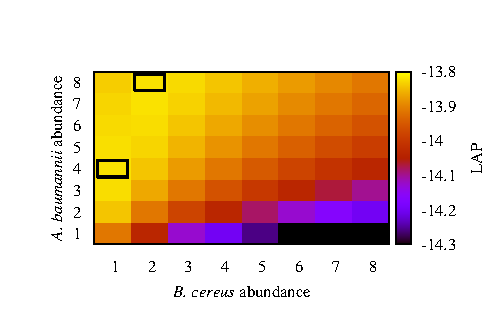
\includegraphics[width=4in]{ref_abun_1} \label{fig:ref_abun_1}}
\hfil
\subfigure[\emph{B. cereus} (4 copies, 5.2MB) and \emph{A. odontolyticus} (7 copies, 2.4MB)]{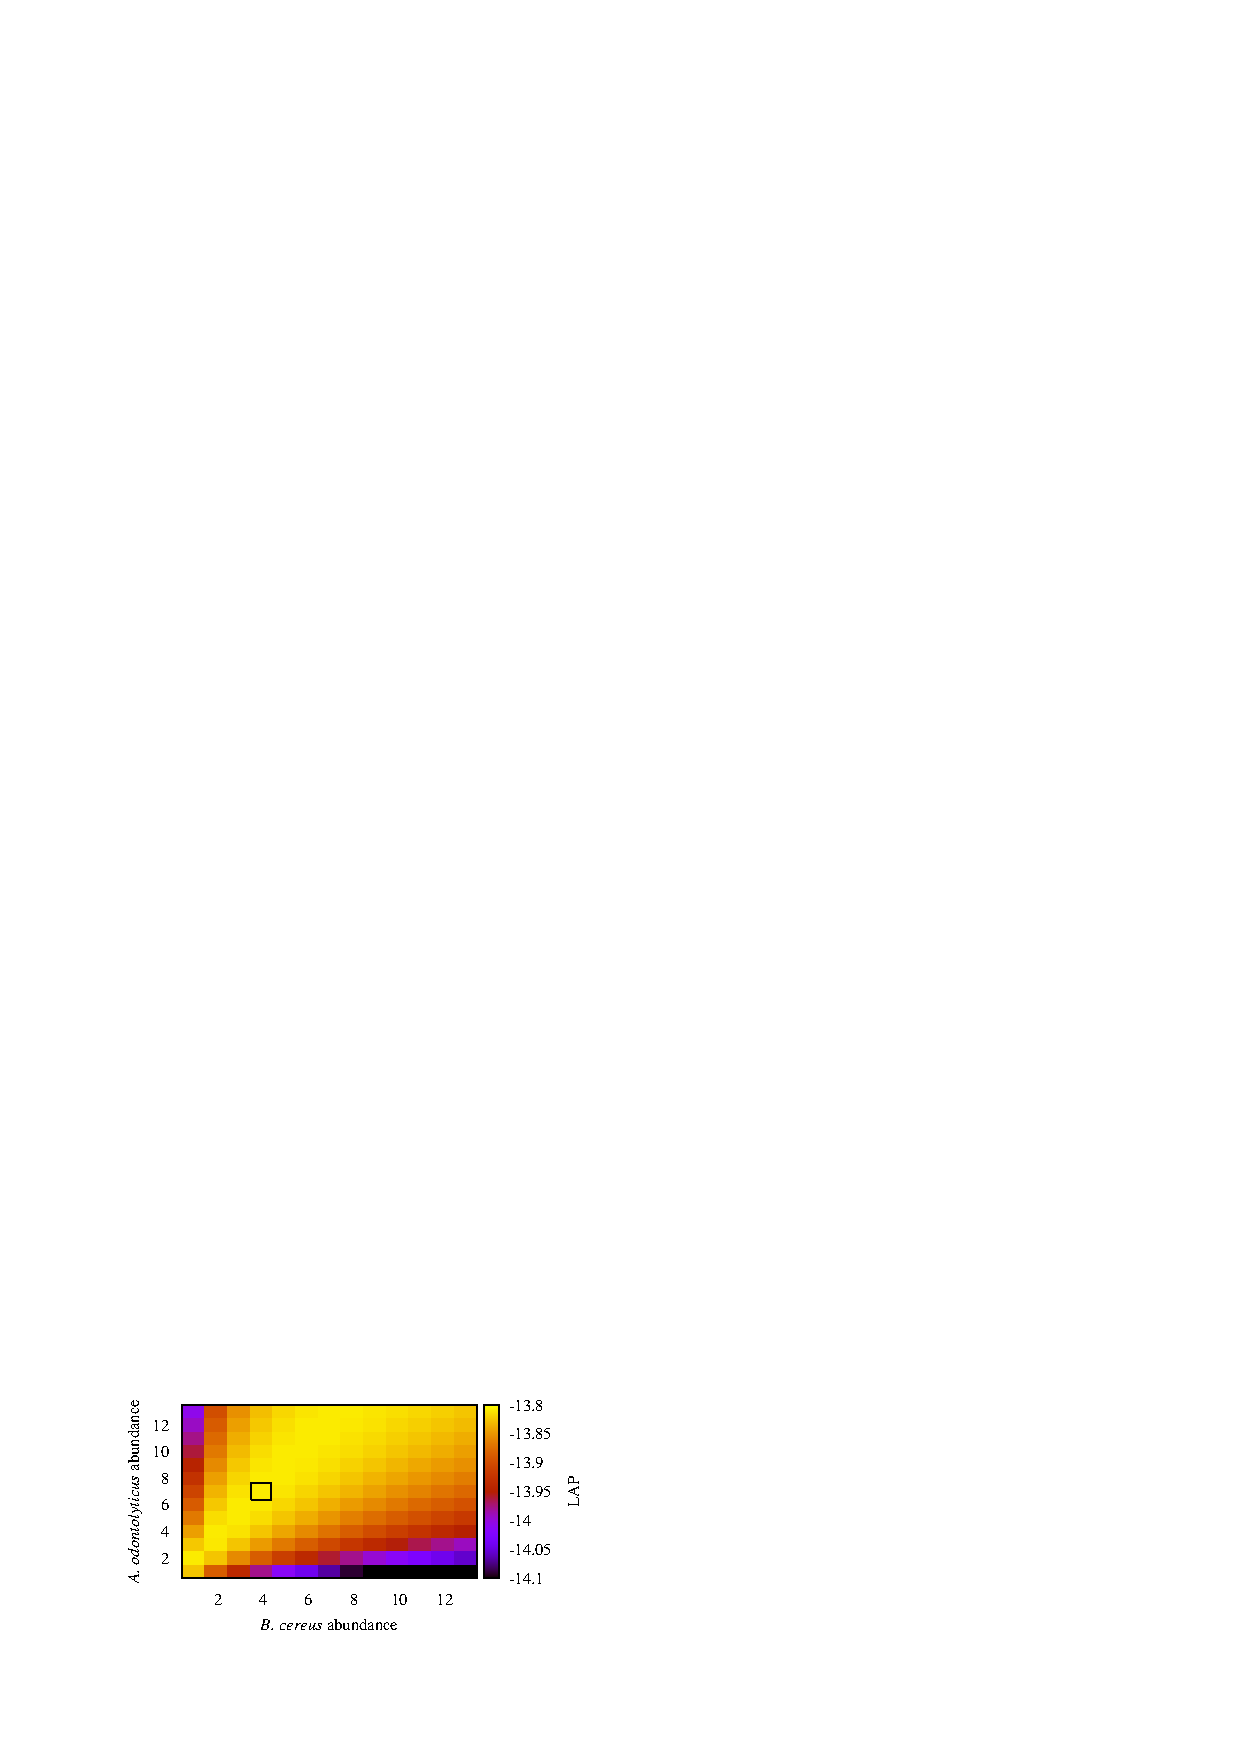
\includegraphics[width=4in]{ref_abun_2} \label{fig:ref_abun_2}}
\end{center}
\renewcommand{\baselinestretch}{1}
\small\normalsize
\begin{quote}
\caption[LAP scores for simulated metagenomic communities.] {LAP scores for simulated metagenomic communities. Each cell (x,y) represents the LAP score for a mixture of \emph{x} copies of the x-label bacteria and \emph{y} copies of the y-label bacteria.  In both groups, the true abundance ratios maximize the LAP score (indicated by a black rectangle in respective plots). \label{fig:ref_abun}}
\end{quote}
\end{figure}
\renewcommand{\baselinestretch}{2}
\small\normalsize
\newpage

\subsection{Extending LAP to metagenomic assemblies}

An important simplifying assumption of our framework is that the sequencing process is uniform in coverage.
In metagenomics, however, the relative abundances of organisms are rarely uniform~\cite{carrigg2007dna,krsek1999comparison,morgan2010metagenomic,temperton2009bias}, reflecting the difference in abundance between the different organisms within a community.
Here we show that taking this abundance information into account allows us to extend the LAP framework to metagenomic data.
%This feature makes using the LAP score incorrect out of the box.
%Later steps in the pipelines often deal with abundance estimation and phylogenetic classification.
We now assume that while the abundances of each organism may vary dramatically, the sequencing process still has uniform coverage across the \emph{entire} community.
%It is important to note while the abundances of each organism may vary dramatically, the sequencing process still produces a uniform coverage of the complete environment.
For example, consider a simple community containing two organisms (A and B), one which is twice as abundant as the other.
This community, thus, comprises twice as much of A's DNA than that of B.
Assume, for simplicity, that the community contains exactly three chromosomes (two of A and one of B).
A random sequencing process would sample each of these equally, and an ideal metagenomic assembler would produce two contigs, one covered twice as deep as the other.
%the case where we have three bacteria in an environment (1 copy of strain \emph{A}, 2 copies of strain \emph{B}).
%Now, lets assume we performed enough sequencing to produce a 1x coverage of each individual bacterium.
%An assembler would only output both bacteria strains, despite the difference in coverage.



In essence, we view the collection of individual genomes and their relative abundances as a single \emph{metagenome} where each genome is duplicated based on their abundance (\figurename \ref{fig:metagenome}).
%Thus, we now assume we have uniform coverage across the entire metagenome.
This setting is similar to that of repeats in single genome assembly, where a repetitive element can now include an entire genome.
Like in the case of single genomes, the assembler that correctly estimates these repeat counts maximizes the LAP score.
In other words, in order to accurately evaluate the metagenomic assemblies using our LAP framework, the abundance (or copy number) of each contig is needed.
%The assembler that figures out the correct copy number of repeats (in this case, contigs) will have the highest LAP score.
As most metagenomic assemblers do not report this information,
here we use the average coverage of the contig (provided by the MetAMOS pipeline) to represent the copy number.

%In order to accurately calculate the LAP of a metagenomic assembly, in addition to the actual assemblies, we need the abundances.
In the error-free model, we compute the probability of a read, $p_r$, given the assembled sequence and abundance as:
%
\begin{equation}
  \label{meta_read_probability}
  p_r = \frac{\sum_{c \in \text{Contigs}}\text{abun}(c)*n_{rc}}{2\hat{L}}
\end{equation}
%
\begin{equation}
  \label{meta_read_length}
  \hat{L} = \sum_{c \in \text{Contigs}}\text{abun}(c)*L_{c}
\end{equation}
%
where $\text{abun}(c)$ is the abundance of contig c, $n_{rc}$ is the number of times read $r$ occurs in contig $c$, and $\hat{L}$ is the adjusted total assembly length.  In the case where the abundance of each contig is 1, calculating $p_r$ is identical to the original LAP (single genome) formulation.  A similar modification can be done to handle sequencing errors outlined in \cite{LAP}.

Our prior work has shown we can approximate the probabilities using fast and memory efficient search alignment programs (e.g., Bowtie2~\cite{langmead2012fast}) when it is impractical to calculate the exact probabilities for large read sets.
We can apply the metagenomics modification above to the alignment tool-based method:
%
\begin{equation}
\label{}
p_{r} = \frac{\sum_{j \in S_r} \text{abun}(j_{\text{contig}})*p_{r,j_{\text{subs}}}}{2\hat{L}}
\end{equation}
where $S_r$ is the set of alignments in the SAM file for the read $r$ and the probability of alignment, $p_{r,j_{\text{subs}}}$, is approximated by $\epsilon^{subs}(1 - \epsilon)^{l - subs}$ where $\epsilon$ is the probability of an error (a mismatch, an insertion, or a deletion).



%allow the assembler to tell us what copy number it expects for each contig - that is the average coverage for the contig (provided in our analysis by the MetAMOS pipeline).
%Our LAP framework uses the average per basepair coverage of assembled contigs provided by MetAMOS.

An important factor in any likelihood-based assembly evaluation framework is the handling of reads that do not align well to the given assembly.
In practice, unalignable reads are often the result of sequencing errors and contaminants.
If these reads are given a probability close to 0, then the best assembler would be the one that incorporates the most reads.
In our original LAP framework, a read that does not align well does not decrease the overall assembly probability more than the probability of an assembly that contains the appended read as an independent contig.
This does not change when we handle metagenomic data, since the average coverage of the ``new'' contig is one.

%However, commonly used metagenomic abundance tools are often targeted at taxonomic classification~\cite{segata2012metagenomic,brady2009phymm,liu2010metaphyler,huson2007megan}.
%One strategy to estimate contig abundances is to first perform taxonomic classification on the reads and then align the contigs with the taxonomic database, transitively applying the taxonomic abundances to the contigs.
%In lieu of taxonomic abundances, our LAP framework uses the average per basepair coverage of assembled contigs provided by MetAMOS.
%We use modified version of Sailfish\cite{sailfish}, a tool to quickly calculate transcript abundances using RNA-seq data, to estimate contig abundances.
%One of the underlying assumptions of Sailfish is that the coverage


% \begin{landscape}
% \renewcommand{\baselinestretch}{1}
% \small\normalsize
%
% \renewcommand{\baselinestretch}{2}
% \small\normalsize
% \end{landscape}

\begin{landscape}
\renewcommand{\baselinestretch}{1}
\small\normalsize

\begin{table}[tbp]
\renewcommand{\arraystretch}{1.2}
\centering
\scriptsize
\begin{tabular}{{l}{l}{c}{c}{c}{c}{c}{c}{c}{c}{c}{c}{c}}
\hline
\bfseries Dataset & \bfseries Assembler & \bfseries LAP & \bfseries \#ctgs &  \bfseries Good ctgs & \bfseries Total aln & \bfseries Slt & \bfseries Hvy & \bfseries Ch & \bfseries Size @ 10 Mbp &\bfseries Max ctg size & \bfseries Err per Mbp & \bfseries Aligned reads \\
\hline\hline

mockE & SOAPdenovo & \textbf{-27.031} & 63107 & \textbf{99.3\%} & \textbf{51} & \textbf{166} & 131          & \textbf{1} & 28,208          & 249,819          & \textbf{5.8}  & \textbf{85.75\%} \\
mockE & Velvet     & -28.537          & 12,830 & 96.2\%          & 41          & 256          & \textbf{100} & 2          & 42,269          & 179,673          & 8.7  & 83.30\%        \\
mockE & MetaVelvet & -27.102          & 22,772 & 96.8\%          & 49          & 462          & 156          & 4          & \textbf{62,138} & \textbf{367,458} & 12.7    & 85.65\%      \\
mockE & Meta-IDBA  & -31.166          & 22,032 & 95.4\%          & 47          & 362          & 151          & 3          & 26,141          & 249,069          & 11  & 81.81\%\\
\\
mockS & SOAPdenovo & -60.161          & 44,928 & \textbf{98.8\%} & \textbf{28} & 135          & 98           & \textbf{0} & 5,672           & 186,064          & \textbf{8.3} & 69.78\%  \\
mockS & Velvet     & -60.711          & 21,050 & 95.8\%          & \textbf{28} & 485          & 115          & 1          & 6,060           & 119,120          & 21.5          & 67.26\% \\
mockS & MetaVelvet & -60.442          & 20,551 & 95.3\%          & \textbf{28} & 517          & 143          & 3          & 6,685           & \textbf{217,330} & 20.1         & 67.72\% \\
mockS & Meta-IDBA  & \textbf{-58.851} & 4,559  & 92.5\%          & 18          & \textbf{101} & \textbf{83}  & \textbf{0} & \textbf{13,150} & 119,604          & 10.2  & \textbf{70.67\%}\\
\\
Tongue  & SOAPdenovo & \textbf{-13.844} & 35,230 & \textbf{89.10\%} & \textbf{11} & 1,138 & 2,618 & \textbf{0} & 11,359 & \textbf{238,051} & \textbf{341.5} & \textbf{88.14\%}\\
Tongue  & Meta-IDBA & -21.368 & 25,698 & 88.70\% & 7 & \textbf{710} & \textbf{2,087} & \textbf{0} & 4,215 & 59,188 & 399.6 & 58.89\% \\

\hline
\end{tabular}
\caption[Comparison of assembly statistics for HMP mock Even and mock Staggered datasets]{Comparison of assembly statistics for HMP mock Even and mock Staggered datasets.Numbers in bold represent the best value for the specific dataset.}
\label{tab:hmp}
\end{table}

\renewcommand{\baselinestretch}{2}
\small\normalsize
\end{landscape}


\subsection{Integration into MetAMOS}

In addition to being a standalone framework, the software implementing our metagenomic LAP approach comes packaged with the MetAMOS pipeline.
This allows users the option to run MetAMOS with different assemblers and have our framework automatically select the assembly with the highest LAP score without any prior knowledge from the user.
The first step of the MetAMOS pipeline is to \verb!Preprocess! the reads, optionally filtering out low quality reads.
Those reads are used by the next step \verb!Assemble!.
Users specify the desired assembler using the \verb!-a! parameter of \verb!runPipeline!.
We modified MetAMOS so users can now specify multiple assemblers (comma-separated) after the \verb!-a! parameter, and \verb!runPipeline! will run all assemblers and select the assembly yielding the highest LAP score to be used in downstream analyses.
%The software implementing our approach is made available, open-source and free of charge, at: \url{http://assembly-eval.sourceforge.net/} and with the MetAMOS package: \url{https://github.com/treangen/MetAMOS}.


\section{Results}
\subsection{Likelihood score maximized using correct abundances}
A key property of our framework is that the correct copy numbers (abundances) and assemblies maximizes our LAP score.
To illustrate this property, we simulated two metagenomic communities and calculated the LAP of the reference genomes with a combination of abundances.
The first simulated community consisted of \emph{Bacillus cereus} and \emph{Acinetobacter baumannii} at a ratio of 1:4.
We generated 200bp reads at 20x coverage of the metagenome (20x of \emph{B. cereus} and 80x of \emph{A baumannii}).
We calculated the LAP scores of the error-free reference genomes for all combinations of abundances (ranging from 1 copy to 8 copies) for each bacteria.
%We calculated the LAP score on error-free reference assemblies with all combinations of abundances from 1 copy to 8 copies for each bacteria.
The second simulated community consisted of \emph{Bacillus cereus} and \emph{Actinomyces odontolyticus} at a ratio of 4:7.
We generated 200bp reads at 20x coverage of the metagenome (80x of \emph{B. cereus} and 140x of \emph{A odontolyticus}).
We calculated the LAP scores of the error-free reference genomes for all combinations of abundances (ranging from 1 copy to 13 copies) for each bacteria.


%\begin{figure}[!t]
%\centering
%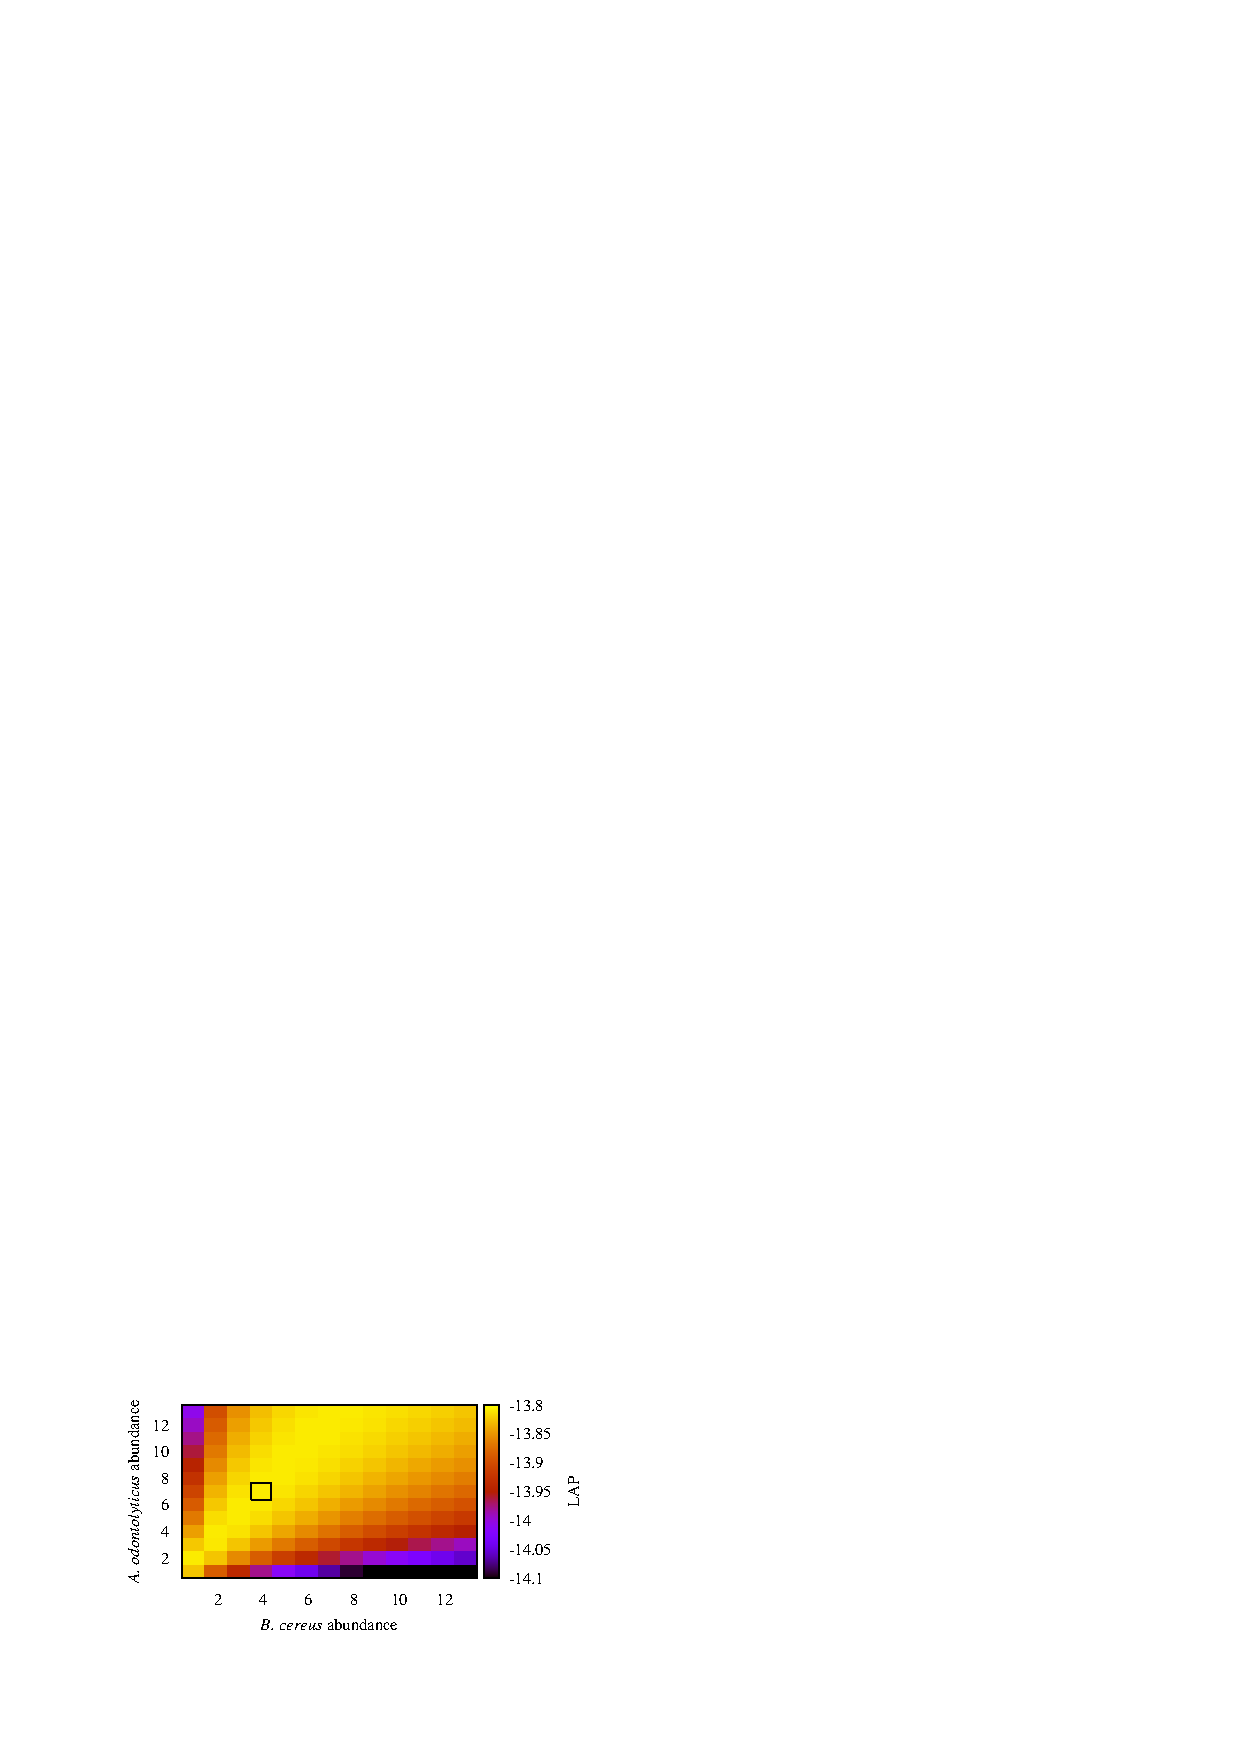
\includegraphics[width=3in]{ref_abun_2}
% where an .eps filename suffix will be assumed under latex,
% and a .pdf suffix will be assumed for pdflatex; or what has been declared
% via \DeclareGraphicsExtensions.
%\caption{LAP scores for simulated B. cereus (4x, 5.2MB) and A. odontolyticus (7x, 2.4MB)}
%\label{fig:ref_abun_2}
%\end{figure}

We expect the highest LAP scores for the assemblies that contain the correct abundance ratios (1:4 or 2:8 in the first community, and 4:7 in the second community).
%1:4 , 2:8 boxes to be highest in figure A, and 4:7, 8:14, etc. in panel 2.  Y
As seen in Figs. \ref{fig:ref_abun_1} and \ref{fig:ref_abun_2}, our LAP score is able to accurately reflect the varying organism abundance ratios present in the sample.
The LAP score increases as the estimates approach the true abundance ratios, with the true ratio yielding the highest LAP scores in both communities.

\begin{figure}[htb!]
\begin{center}
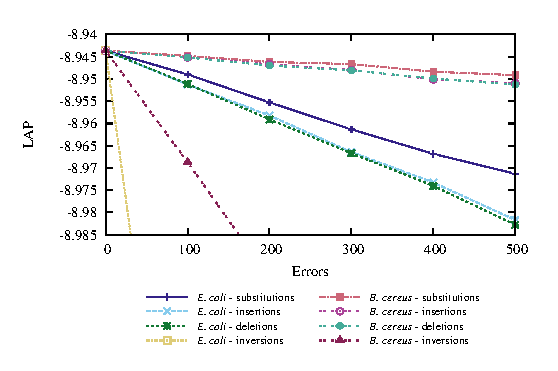
\includegraphics[width=.8\textwidth]{errors}
\end{center}
\renewcommand{\baselinestretch}{1}
\small\normalsize
\begin{quote}
\caption[Synthetic errors in simulated \emph{E. coli} and \emph{B. cereus} (1 copy, 5.2Mbp) community]{Synthetic errors in simulated \emph{E. coli} (5 copies, 4.9Mbp) \emph{B. cereus} (1 copy, 5.2Mbp) community.}
\label{fig:errors}
\end{quote}
\end{figure}
\renewcommand{\baselinestretch}{2}
\small\normalsize

\subsection{Impact of errors on synthetic metagenomes}

One of the often overlooked aspects of metagenomic assembly evaluation is the weighing of errors that occur in contigs with different abundances.
%In single genome assembly, errors are often not weighted since the genome has uniform coverage.
%When detecting errors with the aid of a reference, all substitution errors occurring within a genome are weighted the same (ignoring additional information, such as whether it occurs in a genic or regulatory element).
%When organism abundances are uniform, the weight of an assembly error is also uniform.
In metagenomic samples the relative organism abundances can vary by orders of magnitudes.
A typical reference-based evaluation would equally weight the errors irrespective of the abundance of the erroneous contigs.
The proposed metagenomic LAP score, however, automatically handles this situation and appropriately weighs errors according to genome abundance.
%Thus, errors in highly abundant organisms will have more of an impact on the LAP score than errors in organism of lower abundance.
To illustrate this, we simulated a small metagenomic community consisting of \emph{Escherichia coli} and \emph{Bacillus cereus} at a 5:1 ratio.
We introduced an increasing number of common assembly errors (single-base substitutions, insertions, deletions, and inversions) into the two organisms assemblies and observed the resulting LAP score.

As shown in \figurename \ref{fig:errors}, the higher the number of synthetic errors, the lower the LAP score.
Insertions/deletions were more deleterious to the LAP score than substitutions, since in addition to causing a mismatch, an insertion/deletion changes the overall genome size.
Although inversions did not change the overall genome size (and would therefore not be detected by simplistic measures such as N50), these errors had the greatest impact on the LAP score because they prevented the alignment of reads across the boundaries of the inversions.
%With substitutions and indels, reads were still able to align across the error and only incurred the additional mismatch penalty.
%Conversely, read alignment tools will fail to detect read alignments that span the borders of the inversions.

%Whereas substitutions, insertions, and deletions still allowed reads to align albeit with a lower probability, reads that inversions are essentially treated as complete

As expected, errors introduced into the more abundant organism, \emph{E. coli}, had a greater affect on the LAP score than those inserted into \emph{B. cereus}.
Our LAP score was able to accurately weigh the errors by the abundance of each organism.


\subsection{Likelihood scores correlate with reference-based metrics}
%c|c|c|c|c|c


With real metagenomic samples, it is difficult to make evaluations given the lack of high quality references.
Using purely simulated data has the issue of not accurately capturing the error and bias introduced by sequencing technology.
Thus, to evaluate our LAP score, we use two `mock' communities (Even and Staggered) provided by the Human Microbiome Project (HMP) consortium\cite{mitreva2012structure,methe2012framework}.
These communities were created using specific DNA sequences from organisms with known reference genomes (consisting of over 20 bacterial genomes and a few eukaryotes) and abundances.
The mock Even community consisted of 100,000 16S copies per organism per aliquot, while the mock Staggered community consisted of 1,000 to 1,000,000 16S copies per organism per aliquot.
Data used from the HMP mock communities are available at \url{http://www.ncbi.nlm.nih.gov/bioproject/48475}.
We calculated the LAP score on assemblies produced by MetAMOS~\cite{treangen2013metamos} using several assemblers: SOAPdenovo~\cite{SOAPdenovo}, Metavelvet~\cite{namiki2012metavelvet}, Velvet~\cite{Velvet}, and Meta-IDBA~\cite{peng2011meta}.
The additional \emph{de novo} and reference-based metrics for the assemblies were taken from MetAMOS~\cite{treangen2013metamos}.  These metrics include:
   \begin{itemize}
   \item number contigs (\# ctgs) -- total number of contigs/scaffolds in the assembly
   \item good contigs (Good Ctgs) -- fraction of contigs that mapped without errors to reference genomes
   \item total aligned (Total aln) -- total amount of sequence (in Mbp) that can be aligned to the reference genomes
   \item slight mis-assemblies (Slt) -- alignments that cover 80\% or more of the aligned contig in a single match (Slt)
   \item heavy misassemblies (Hvy) -- alignments that cover less than 80\% of the aligned contig in a single match or have two or more matches to a single reference
   \item chimeras (Ch) -- contigs with matches to two distinct reference genomes
   \item size at 10 megabases (Size @ 10 Mbp) - the size of the largest contig $c$ such that the sum of all contigs larger than $c$ is more than 10 Mbp (similar to the commonly used N50 size)
   \item max contig size (Max ctg size) -- size of the largest contig in the assembly
   \item errors per megabase (Err per Mbp) -- average number of errors per Mbp in the assembly
   \end{itemize}

Generally, the \emph{de novo} LAP scores agree with the referenced-based metrics (Table \ref{tab:hmp}).
In the mock Even dataset, SOAPdenovo has the greatest LAP score, the highest fraction of contigs that can align to a reference genome without error, total amount of sequence that can be aligned to a reference genome, while also having the lowest amount of misassemblies (including chimeric) and errors per Mbp.
It is important to note that if user selected an assembly based on the best contiguity at 10Mbp, they would select the MetaVelvet assembly, which contains double the error rate per Mbp as the SOAPdenovo assembly while aligning 2Mbp less to the references.

\begin{figure}[tb!]
\begin{center}
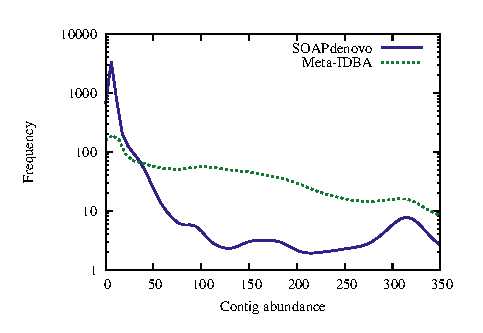
\includegraphics[width=.8\textwidth]{coverage}
\end{center}
\renewcommand{\baselinestretch}{1}
\small\normalsize
\begin{quote}
\caption[Frequency of contig abundances for assemblies of the HMP mock Staggered dataset]{Frequency of contig abundances for assemblies of the HMP mock Staggered dataset.}
\label{fig:coverage}
\end{quote}
\end{figure}
\renewcommand{\baselinestretch}{2}
\small\normalsize

Since the abundances of each organism in the mock Even dataset are fairly similar, the mock Staggered abundance distribution creates a more realistic scenario encountered in metagenomic environments.
Here, the Meta-IDBA assembly has the greatest LAP score, but aligns roughly a third less sequences to the reference genomes than SOAPdenovo.
The Meta-IDBA assembly contains approximately a tenth of the amount of contigs (4,559 vs. 44,928) as SOAPdenovo.
The SOAPdenovo assembly contains a greater number of contigs at a very low abundance (\figurename \ref{fig:coverage}).
On large contigs Meta-IDBA performs better than SOAPdenovo and has a lower error rate (see \figurename 4 in \cite{treangen2013metamos}).
However, Meta-IDBA assembles a smaller fraction of the low-abundance genomes than SOAPdenovo, leading fewer sequences to align.
The LAP score penalizes misassemblies within abundant contigs in the SOAPdenovo results.


%Given how the mock Staggered community was constructed (each ratio of 16S copies per aliquot occurred roughly the same number of times), the frequency of contig abundances should be approximately uniform for the community.
%The SOAPdenovo assembly was able to align more reads, but the reads were localized in these low coverage regions.
%The distribution of contig abundances in the Meta-IDBA assembly was closer to the expected distribution than the SOAPdenovo assembly.

%The Meta-IDBA assembly a far more uniform frequency of contig abundances compared to the SOAPdenovo assembly.

Next, we applied our framework on real data where we did not know the actual genomes comprising the sample (HMP tongue dorsum female sample, SRS077736) (Table \ref{tab:hmp}).
Although we do not know for certain which organisms are present in the sample, the HMP identified a reference genome set with high similarity to the sequences within the sample (HMP Shotgun Community profiling SRS077736).
The reference-based error metrics only consider chimeric errors due to the possibility of structural difference between an organism and its version in the reference database.
We calculated the LAP of the assemblies using a single library consisting of 42,013,917 reads.
The SOAPdenovo assembly had a far greater LAP score than the Meta-IDBA assembly.
The higher score is due to the SOAPdenovo assembly recruiting more reads (88.14\% to 58.89\%) in relation to its genome size (46Mbp to 37Mbp) than the Meta-IDBA assembly.
Furthermore, the MetAMOS metrics show that the SOAPdenovo assembly contained approximately 60 less errors per Mbp than the Meta-IDBA assembly.

%These datasets have the advantage over simulated data because it captures the error and bias introduced from the sequence technology.


\renewcommand{\baselinestretch}{1}
\small\normalsize

\begin{table}[tb!]
\label{tab:metamos_lap}
\centering
\begin{tabular}{{l}{c}{c}{c}{c}}
\hline
\bfseries Assembler & \bfseries Contigs & \bfseries LAP & \bfseries N50 (Kbp) & \bfseries  Errors \\
\hline \hline
newbler  & \bf{1} & \bf{-13.064} & \bf{156} & 1 \\
SOAPdenovo & 23 & -14.238 & 9 & \bf{3} \\
Velvet & 3 & -13.157 & 92 & \bf{0} \\
MetaVelvet & 3 & -13.157 & 92 & \bf{0} \\
\hline
\end{tabular}
\caption[Self-tuning MetAMOS using \emph{C. ruddii} test dataset]{Self-tuning MetAMOS using \emph{C. ruddii} test dataset.}
\end{table}

\renewcommand{\baselinestretch}{2}
\small\normalsize

\subsection{Tuning assembly parameters for MetAMOS}
Assemblathon1~\cite{earl2011assemblathon} has shown that assembly experts can often get drastically different assemblies using the same assemblers, highlighting the difficulty of choosing the \emph{right} parameters for a given assembler.
Our metagenomic LAP framework comes packaged with the MetAMOS pipeline, allowing users the option to run MetAMOS with different assemblers and automatically select the assembly with the highest LAP score.
This step occurs without any prior knowledge from the user.

We showcase the ease of use of the automated assembler selection within MetAMOS using the \emph{Carsonella ruddii} (156Kbp) dataset packaged with MetAMOS (Table ~\ref{tab:metamos_lap}).
Errors were found using DNADIFF~\cite{phillippy2008genome} and MUMmer~\cite{delcher2003using}.
The newbler assembly produced one contig containing the complete \emph{C. ruddii} genome.
The SOAPdenovo assembly produced a severely fragmented assembly with the most number of errors.
The MetaVelvet and Velvet produced identical assemblies, containing 3 contigs of sizes 92Kbp, 65Kbp, and 1.7Kbp, but contained an additional 158bp compared to the \emph{C. ruddii} genome.
Upon closer inspection, there were overlaps between the contigs ranging from 38bp to 73bp.
This is not surprising given MetaVelvet's and Velvet's de bruijn graph-based approach could not resolve repetitive regions between the contigs.
Newbler, on the other hand, contained only a single insertion error.
The LAP score of the Newbler assembly was greater due to more reads being able to align across the regions that were broken apart in the MetaVelvet and Velvet assemblies.
Additionally, the Newbler assembly did not contain the duplicated sequence found in the other assemblies.
MetAMOS was able to select the most likely assembly without requiring any additional input from the user.

\section{Discussion}

In this paper, we have proposed an extension to our LAP framework to perform \emph{de novo} comparisons of metagenomic assemblies.
Unlike traditional \emph{de novo} metrics used for measuring assembly quality, our extended LAP score correlates well with reference-based measures of metagenomic assembly quality.
However, in this study, we have realized that there is a lack of reference-based metrics when evaluating metagenomic assemblies.
Misjoins betweens organisms may be more deleterious than misjoins within a single genome.
Furthermore, current reference-based metrics do not take into account the relative abundances of the organisms when evaluating metagenomic assemblies.
The metrics provided by MetAMOS do not factor in the contig abundances when examining assembly errors.
This made it difficult to compare our LAP score to their reference-based metrics because, intuitively, an error in a highly abundant organism should be \emph{worse} than an error in a rare, low coverage organism.
Our LAP score implicitly weighs the errors in abundant contigs more than those in lesser abundant contigs.
In our results, we have proposed one such reference-based metric that scales the errors by the relative abundance of the contig it occurs within.

It is important to note that we have only focused on the complete reconstruction of the metagenome from the set of reads.
Assembly algorithms are designed with specific biological applications in mind, such as, the conservative reconstruction of the genic regions.
Studies focusing on the genic regions may tolerate large-scale rearrangements as long as the genic regions were correctly assembled.
Conversely, other studies may want to focus on the reconstruction and detection of rare pathogenic bacteria in an environment.
These application specific assembly algorithms all attempt to optimize their formulation of the assembly problem.

Our metagenomic LAP extension relies heavily on the idea that the sequencing process of the metagenome is roughly uniform, and that the reads are independently sampled from the genome.
Biases exist in all steps of the sequencing process, from the extraction of DNA from organisms with different cell membranes/walls~\cite{carrigg2007dna,krsek1999comparison} to the sequencing protocol used~\cite{morgan2010metagenomic,temperton2009bias}.
In the future, we would like to implement a more specific model that better captures the sequencing process.

%De novo metric, more misleading in assemblies -> chimera

%We would like to stress that \emph{de novo} measures of assembly quality, such as ours, are critically needed by researchers attempting to assemble of yet unknown genomes.

Results from GAGE~\cite{salzberg2011gage} and Assemblathon~\cite{earl2011assemblathon,bradnam2013assemblathon} have shown that the specific characteristics of the data being assembled has a great impact on the performance of the assembler.
This problem is magnified in metagenomic assembly.
By integrating our LAP framework in MetAMOS, we have allowed researchers to accurately and effortlessly run and evaluate assemblies without any prior knowledge on evaluating assembly quality.

In our framework, we use the average coverage of the contig (provided by MetAMOS) to estimate abundance.
There are issues with this measure as it is possible that mis-assembled repeats within a contig will affect our estimate of depth of coverage and could impact our underlying statistics.
A better approach is to use something more robust than the mean coverage, such as the median coverage, to avoid being influenced by such regions.
While the user can supply the median coverage to our standalone framework, future work includes building this feature into MetAMOS.
Another approach involves breaking contigs at regions of differing coverage (using tools such as AMOSvalidate\cite{phillippy2008genome}), so there will be less deviation in the average coverage within the contig.

It should be noted that in some cases it may not be tractable to run the complete collection of assemblers with MetAMOS.
In such cases, we should first employ heuristics (such as \cite{chikhi2013informed}) to aid in selecting potential assemblers (and parameters) to run.
For the assembler selection process, we can use the LAP framework's sampling procedure in combination with calculating read probabilities in parallel to reduce runtime.

Our goal was to provide a global measure of how good a metagenomic assembly may be, not to detect assembly errors.
Other likelihood-based frameworks, such as ALE, use frequencies of certain sequences to aid in detection of possible chimeric contigs.
We are able to apply similar modifications to our LAP framework to find regions of possible misassembly.
Finally, we plan to extend our framework to give a more detailed breakdown of the LAP scores of segments assembled using the same subset of reads across different assemblies.
The goal would be to take high-scoring assembled segments from individual assemblies to recreate an assembly with overall greater likelihood.
This approach will be of great benefit to the field of metagenomic assembly since assemblers are often designed with different constraints and goals in mind, e.g., low memory footprint, assembling high/low coverage organisms, or tolerating population polymorphisms.
For example, on the mock Staggered dataset, Meta-IDBA best assembled the most abundant genomes while SOAPdenovo had a better representation of the low abundance organisms.
Providing a systematic way of combining assembler approaches using our LAP score will produce better assemblies for downstream analyses.


% An example of a floating figure using the graphicx package.
% Note that \label must occur AFTER (or within) \caption.
% For figures, \caption should occur after the \includegraphics.
% Note that IEEEtran v1.7 and later has special internal code that
% is designed to preserve the operation of \label within \caption
% even when the captionsoff option is in effect. However, because
% of issues like this, it may be the safest practice to put all your
% \label just after \caption rather than within \caption{}.
%
% Reminder: the "draftcls" or "draftclsnofoot", not "draft", class
% option should be used if it is desired that the figures are to be
% displayed while in draft mode.
%
%\begin{figure}[!t]
%\centering
%\includegraphics[width=2.5in]{myfigure}
% where an .eps filename suffix will be assumed under latex,
% and a .pdf suffix will be assumed for pdflatex; or what has been declared
% via \DeclareGraphicsExtensions.
%\caption{Simulation Results}
%\label{fig_sim}
%\end{figure}

% Note that IEEE typically puts floats only at the top, even when this
% results in a large percentage of a column being occupied by floats.


% An example of a double column floating figure using two subfigures.
% (The subfig.sty package must be loaded for this to work.)
% The subfigure \label commands are set within each subfloat command, the
% \label for the overall figure must come after \caption.
% \hfil must be used as a separator to get equal spacing.
% The subfigure.sty package works much the same way, except \subfigure is
% used instead of \subfloat.
%
%\begin{figure*}[!t]
%\centerline{\subfloat[Case I]\includegraphics[width=2.5in]{subfigcase1}%
%\label{fig_first_case}}
%\hfil
%\subfloat[Case II]{\includegraphics[width=2.5in]{subfigcase2}%
%\label{fig_second_case}}}
%\caption{Simulation results}
%\label{fig_sim}
%\end{figure*}
%
% Note that often IEEE papers with subfigures do not employ subfigure
% captions (using the optional argument to \subfloat), but instead will
% reference/describe all of them (a), (b), etc., within the main caption.


% An example of a floating table. Note that, for IEEE style tables, the
% \caption command should come BEFORE the table. Table text will default to
% \footnotesize as IEEE normally uses this smaller font for tables.
% The \label must come after \caption as always.
%
%\begin{table}[!t]
%% increase table row spacing, adjust to taste
%\renewcommand{\arraystretch}{1.3}
% if using array.sty, it might be a good idea to tweak the value of
% \extrarowheight as needed to properly center the text within the cells
%\caption{An Example of a Table}
%\label{table_example}
%\centering
%% Some packages, such as MDW tools, offer better commands for making tables
%% than the plain LaTeX2e tabular which is used here.
%\begin{tabular}{|c||c|}
%\hline
%One & Two\\
%\hline
%Three & Four\\
%\hline
%\end{tabular}
%\end{table}


% Note that IEEE does not put floats in the very first column - or typically
% anywhere on the first page for that matter. Also, in-text middle ("here")
% positioning is not used. Most IEEE journals/conferences use top floats
% exclusively. Note that, LaTeX2e, unlike IEEE journals/conferences, places
% footnotes above bottom floats. This can be corrected via the \fnbelowfloat
% command of the stfloats package.



\section{Conclusion}
In this paper we have described an extension to our \emph{de novo} assembly evaluation framework (LAP) for comparing metagenomic assemblies.
We showed that the true metagenome and correct relative abundances maximizes our extended LAP score.
Furthermore, we have integrated our framework into the metagenomic assembly pipeline MetAMOS, showing that any user is able to reproduce quality evaluations of metagenomic assemblies with relative ease.
